\documentclass{article}
\usepackage{graphicx}
\usepackage{sidecap}
\usepackage{fancyhdr}
\usepackage[absolute]{textpos}
\usepackage{listings}
\usepackage{amsmath}
\usepackage[utf8]{inputenc}
\usepackage[francais]{babel}
\usepackage{sistyle}
\usepackage{amsmath}
\usepackage{hyperref}
\usepackage{color}
\usepackage{adjustbox}
\usepackage{floatrow}
\usepackage{float}
\DeclareCaptionFont{Small}{\fontsize{9}{11}\selectfont}
\usepackage{wrapfig}
\usepackage[bottom]{footmisc}

\usepackage{graphicx}
\usepackage{caption}
\usepackage{float}
\usepackage{sidecap}
\usepackage{fancyhdr}
\usepackage{lscape}
\usepackage{cmap}
\usepackage[T1]{fontenc}   %Allow accent to be copy and pasted correctly
\usepackage[utf8]{inputenc}
\usepackage[francais]{babel}
\usepackage[absolute]{textpos}
\usepackage{url}
\usepackage[top=3cm , bottom=3cm, left=2.5cm , right=2.5cm]{geometry}


\frenchbsetup{StandardItemLabels=true, CompactItemize=false, ReduceListSpacing=true}


\renewcommand{\thepage}{\arabic{page}}
%\setcounter{page}{0}

\addto\captionsfrench{\renewcommand{\figurename}{Image}}



%partie concernant la gestion des entÍtes
\pagestyle{fancy}
%\renewcommand\headrulewidth{1pt}
%\fancyhead[L]{Nicolas Potie}
\renewcommand\footrulewidth{1pt}
\fancyfoot[C]{mécanismes de l'évolutiion biologique: micro-évolution}
\fancyfoot[R]{\thepage}
%fin

\begin{document}
\section{Le modèle Hardy-Weinberg}
Le modèle décrit l'évolution, au sein d'une \textbf{population}, des fréquences alléliques et des fréquences génotypiques, d'une génération à l'autre, en ignorant la plupart des facteurs sources d'évolution. En effet, il fait plusieurs hypothèses non réalistes:

\begin{itemize}
\item Accouplement entre les individus aléatoires (panmixie)
\item Absence de mutation.
\item Absence de migration
\item Taile de la population infinie.
\item Absence de sélection d'individus.
\end{itemize}

On va dans ce document éliminer une à une ces hypothèses pour arriver à un modèle modifié plus réaliste.

Les fréquences des génotypes prédites par le modèle de base pour \textbf{la génération suivante} sont:

\begin{figure}[H]
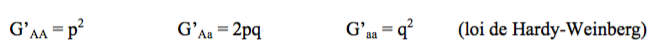
\includegraphics[width=120mm]{./HW.png}
\end{figure}

De plus, notons qu'à l'équilibre Hardy-Weinberg, la fréquence allélique est constante au cours du temps.

\section{Ecart 1: la sélection}

Nous allons définir \textbf{l'aptitude absolue W} d'un génotype. C'est le rapport de la fréquence observée de ce génotype par rapport à sa fréquence attendue sous HW sur bese des fréquences des allèles à la génération précédente.

\begin{itemize}
\item W = 1 $\Rightarrow$ pas d'évolution pour les différents génotypes
\item W > 1 $\Rightarrow$ le génotype est favorisé
\item W < 1 $\Rightarrow$ le génotype est défavorisé
\item W = 0 $\Rightarrow$ le génotype ne se reproduit pas
\end{itemize}

Nous utiliserons plutôt \textbf{l'aptitude relative w (fitness)} qui est le rapport entre l'aptitude absolue d'un génotype et l'aptitude absolue du génotype le plus apte.

Le \textbf{coéfficient de sélection s} est défini en complément de l'aptitude relative.

\begin{equation}
s = 1 - w
\end{equation}

\textbf{Notons enfin qu'un allèle dominant n'est pas forcément le plus apte et qu'un allèle récéssif moins apte.}
\subsection{Sélection contre l'homozygote récessif}

\begin{figure}[H]
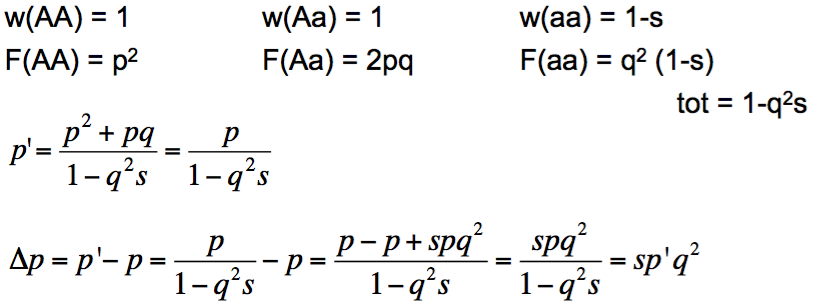
\includegraphics[width=120mm]{./s1.png}
\end{figure}
\pagebreak
Pour calculer la fréquence totale qui sera le dénominateur, il faut additionner les fréquences génotypiques. On sait que les fréquences au total \textbf{valent toujours 1.} Ensuite, on simplifie l'expression.

\begin{figure}[H]
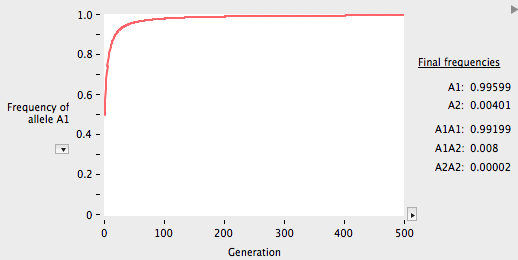
\includegraphics[width=120mm]{./s2.png}
\caption{simulation de la sélection avec w(aa) = 0.5, f(A1) = 0.5}
\end{figure}
Le graphique ci-dessus montre l'impact de la sélection contre l'homozygote récessif. \textbf{L'allèle A2, le récessif, disparait peu à peu du pool génique de la population.} PLus le fitness relatif de aa est faible, plus l'allèle va disparaitre vite. Par ailleurs, la vitesse est grande au debut et ralentis de plus en plus. 


\subsection{Sélection contre les homozygotes (en faveur de l'hétérozygotes)}
\begin{figure}[H]
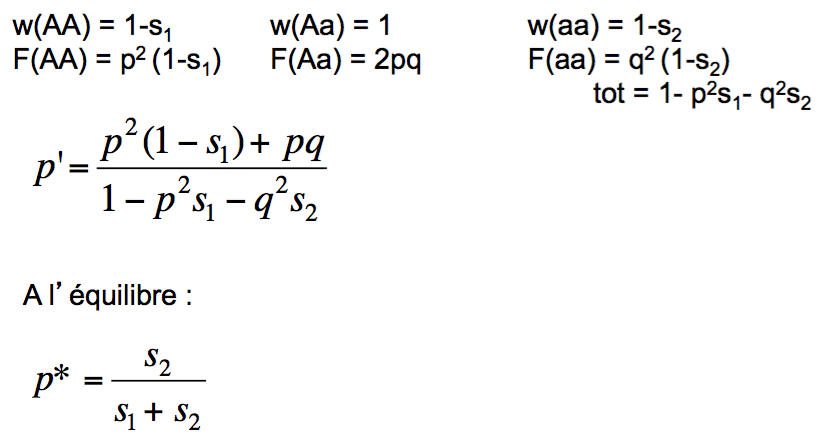
\includegraphics[width=90mm]{./s3.png}
\end{figure}

Dans ce cas-ci, on va atteindre à chaque fois un équilibre stable appelé \textbf{polymorphisme équilibré (hétérosis)}. En effet, on sanctionne les homozygotes mais le pool génétique a de manière équivalente l'allèle récéssif et l'allèle dominant vu que l'hétérozygote est favorisé.

\begin{figure}[H]
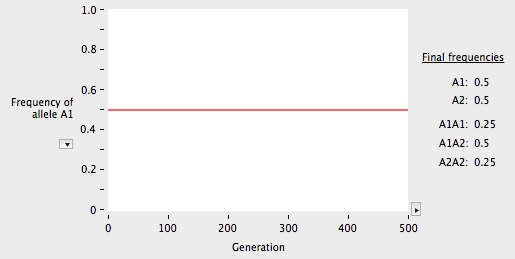
\includegraphics[width=120mm]{./s4.png}
\caption{simulation de la sélection avec w(A1A1) = 0.5, w(A2A2) = 0.5}
\end{figure}

\begin{figure}[H]
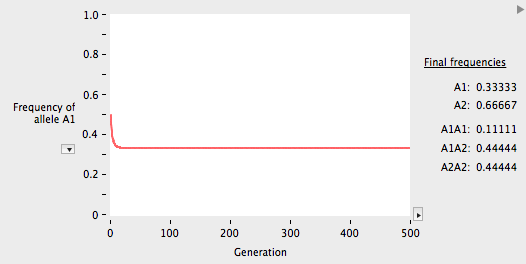
\includegraphics[width=120mm]{./s5.png}
\caption{simulation de la sélection avec w(A1A1) = 0.4, w(A2A2) = 0.7}
\end{figure}

\begin{figure}[H]
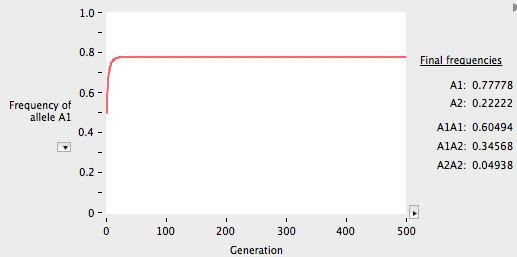
\includegraphics[width=120mm]{./s6.png}
\caption{simulation de la sélection avec w(A1A1) = 0.8, w(A2A2) = 0.3}
\end{figure}


\subsection{Détermination de la valeur d'équilibre de q}
Il existe une valeur de q pour laquelle les pertes de l'allèle récéssif a par sélection sont exactement compensées par les gains de a par mutation.

\begin{equation}
F(A\rightarrow a) = u
\end{equation}

\begin{equation}
F(a\rightarrow A) = v
\end{equation}

le gain de a par mutation est donc égale à pu.

Perte de a par sélection est donnée par:

\begin{equation}
q' = \frac{pq+q^2(1-s)}{1-q^2s}
\end{equation}

\begin{equation}
\Delta q = q' - q =  \frac{pq+q^2(1-s)}{1-q^2s} - q
\end{equation}

L'équilibre est atteint quand:
\begin{equation}
\frac{pq+q^2(1-s)}{1-q^2s} - q = pu
\end{equation}

Ce qui donne:

\begin{equation}
q = q* = \sqrt{\frac{u}{s}}
\end{equation}

\textbf{Si l'allèle récessif est létal, ce qui veut dire que le coéfficient de sélection s est égale à 1}, on a:

\begin{equation}
q = q* = \sqrt{u}
\end{equation}


\subsection{Sélection contre le phénotype dominant}

\begin{figure}[H]
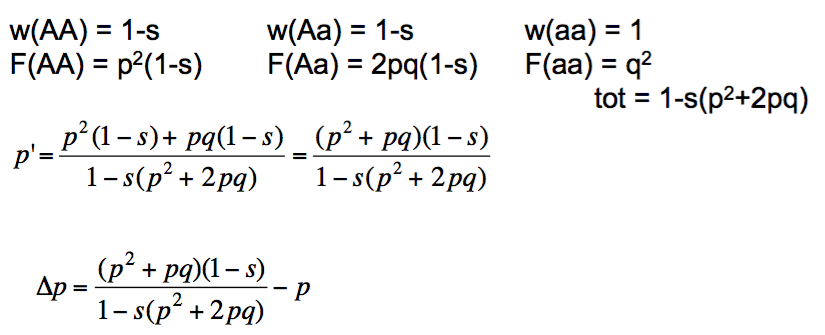
\includegraphics[width=90mm]{./s7.png}
\end{figure}

A l'équilibre, on a:

\begin{equation}
\frac{(p^2+pq)(1-s)}{1-s(p^2+2pq)} - p = qv
\end{equation}

\begin{equation}
p* = \frac{v}{s}
\end{equation}

\begin{figure}[H]
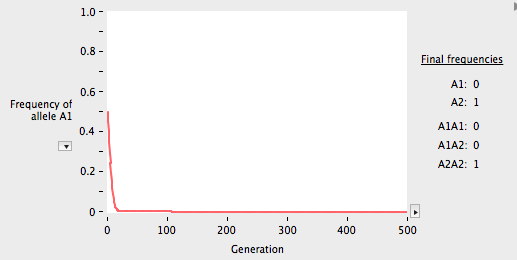
\includegraphics[width=90mm]{./s8.png}
\caption{Simulation de la sélection avec w(A1A1) = 0.7, w(A1A2) = 0.7}
\end{figure}

\begin{figure}[H]
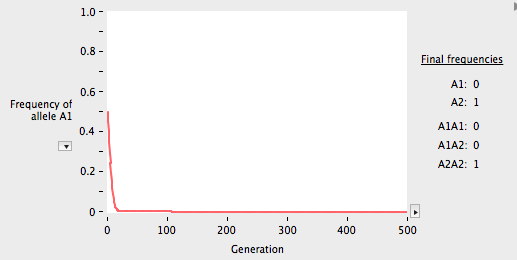
\includegraphics[width=90mm]{./s8.png}
\caption{Simulation de la sélection avec w(A1A1) = 0, w(A1A2) = 0 (létal)}
\end{figure}

On remarque dans les deux cas que \textbf{l'allèle dominant disparait au cours du temps} plus ou moins vite en fonction du fitness des deux génotypes du phénotype dominant.

\subsection{Sélection contre l'hétérozygote}

\begin{figure}[H]
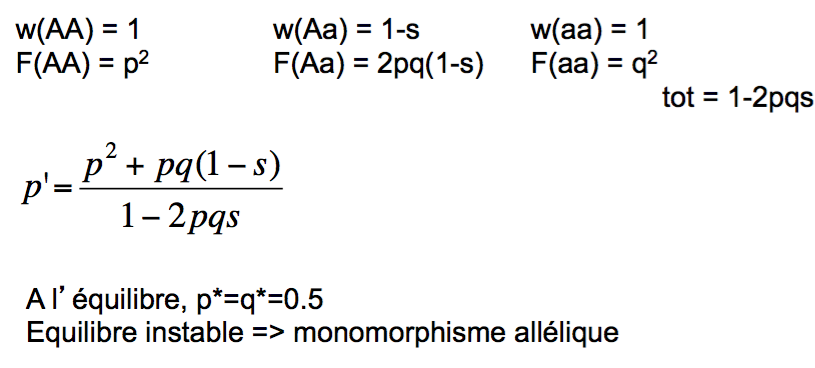
\includegraphics[width=90mm]{./s10.png}
\end{figure}

\begin{figure}[H]
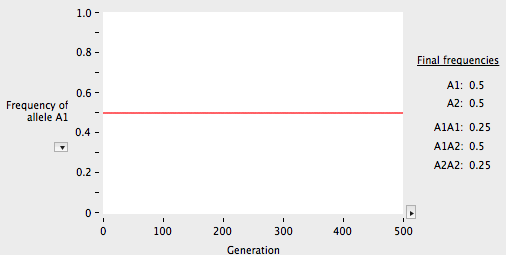
\includegraphics[width=90mm]{./s11.png}
\caption{Simulation de la sélection avec w(A1A2) = 0.3}
\end{figure}

Quelque soit l'aptitude relative de l'hétérozygote, cela va conduire à un \textbf{équilibre instable fait que d'homozygotes d'où un monomorphisme allélique.}

\subsection{Sélection fréquence-dépendante}

La sélection fréquence-dépendante est un mécanisme de sélection des individus par rapport à la fréquence de leur génome dans une population polymorphique. Plusieurs allèles d'un même gène peuvent impliquer des phénotypes différents, aussi bien au niveau purement morphologique que comportemental. Ce qui importe ici est le gain en valeur sélective qui va dépendre de la fréquence des autres phénotypes : un individu avec un phénotype considéré comme "rare" par rapport aux autres individus pourra gagner en survie ou reproduction grâce à cette rareté : on parle alors de sélection fréquence-dépendante négative. C'est-à-dire qu'un individu sera favorisé et aura un gain plus important en fitness si son phénotype est moins fréquent que les autres individus de la population. C'est une des pressions de sélection les plus fortes connues à ce jour, cependant les exemples dans la nature sont assez rares, tout du moins difficilement observables directement.

On peut définir la sélection fréquence dépendante négative de la façon suivante : plus un allèle est répandu dans une population, plus la fitness associée à ce phénotype diminue.

\subsection{Exercices}

\begin{figure}[H]
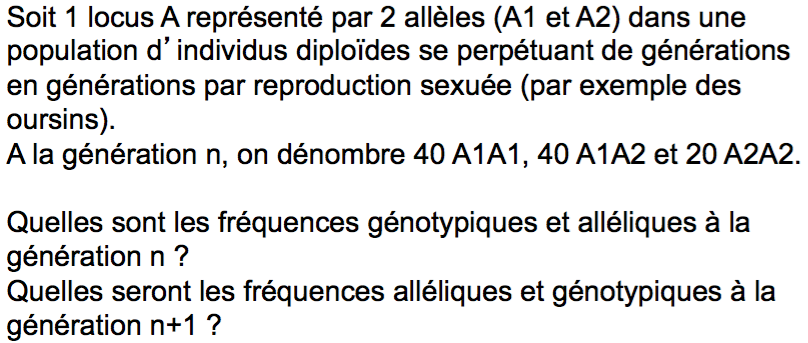
\includegraphics[width=100mm]{./ex1.png}
\end{figure}

On peut calculer les fréquences génotypiques à la génération n:

\begin{equation}
f(A1A1)_{obs} = \frac{40}{100} = 0.4
\end{equation}

\begin{equation}
f(A2A2)_{obs} = \frac{20}{100} = 0.2
\end{equation}

\begin{equation}
f(A1A2) = \frac{40}{100} = 0.4
\end{equation}

Et la fréquence allélique (à la génération n):

\begin{equation}
f(A1) = f(A1A1) + \frac{f(A1A2)}{2} = 0.4 + \frac{0.4}{2} = 0.6
\end{equation}

\begin{equation}
f(A2) = 1-f(A1) = 0.4
\end{equation}

Pour calculer les fréquences génotypiques et allélique à la génération n+1, on va utiliser le modèle Hardy-Weinberg \textbf{en supposant qu'on soit à l'équilibre.}

Nous avons la fréquence allélique, qui ne change pas au cours du temps en cas d'équilibre. Donc,

\begin{equation}
f(A1A1) = p^2 = 0.6 * 0.6 = 0.36
\end{equation}

\begin{equation}
f(A2A2) = q^2 = 0.4*0.4 = 0.16
\end{equation}

Comme on a des accouplements aléatoires, on peut dire que:

\begin{equation}
f(A1A2) = 2pq = 2*0.6*0.4 = 0.48
\end{equation}

\begin{figure}[H]
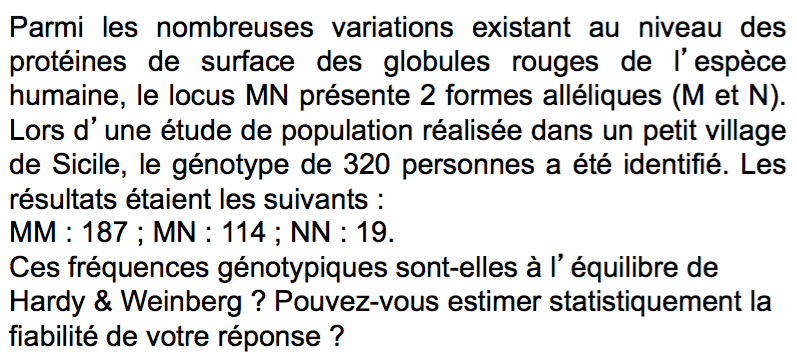
\includegraphics[width=100mm]{./ex2.png}
\end{figure}

Tout d'abord, calculons les fréquences génotypiques à la génération actuelle:

\begin{equation}
f(MM) = \frac{187}{320} = 0.584375
\end{equation}

\begin{equation}
f(MN) = \frac{114}{320} = 0.35625
\end{equation}

\begin{equation}
f(NN) = \frac{19}{320} = 0.059375
\end{equation}

Calculons les fréquences alléliques:

\begin{equation}
f(M) = f(MM) + \frac{f(MN)}{2} = 0.584375 + \frac{0.35625}{2} = 0.7625
\end{equation}

\begin{equation}
f(N) = 1 - f(M) = 1 - 0.7625 = 0.2375
\end{equation}

Pour savoir si la population est à l'équilibre Hardy-Weinberg, il suffit de calculer la fréquence d'hétérozygote attendu dans la population.

\begin{equation}
f_{att}(MN) = 2 * 0.7625 * 0.2375 = 0.3621875
\end{equation}

On remarque que $f_{obs} = 0.35625$ n'est pas égale à la fréquence attendue. La population n'est donc pas forcément à l'équilibre H-W. Néanmoins, il faudrait faire un test de Chi-carré. Il faut pour cela remettre les fréquences attendues en terme d'effectif.

\begin{figure}[H]
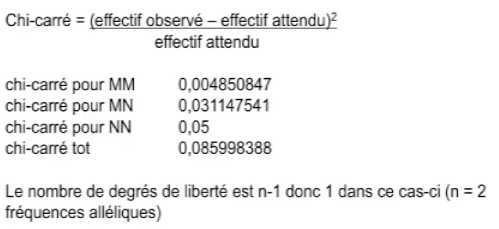
\includegraphics[width=100mm]{./s12.png}
\end{figure}

Il faut ensuite regarder dans la table.


\begin{figure}[H]
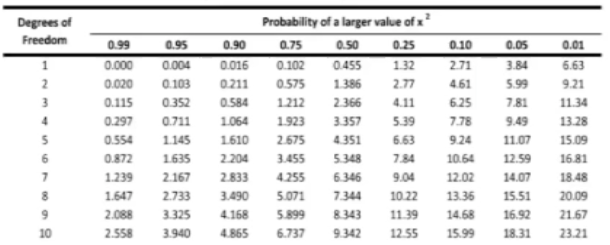
\includegraphics[width=100mm]{./s13.png}
\end{figure}

\begin{figure}[H]
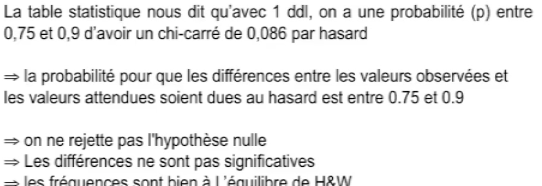
\includegraphics[width=100mm]{./s14.png}
\end{figure}

\pagebreak

\begin{figure}[H]
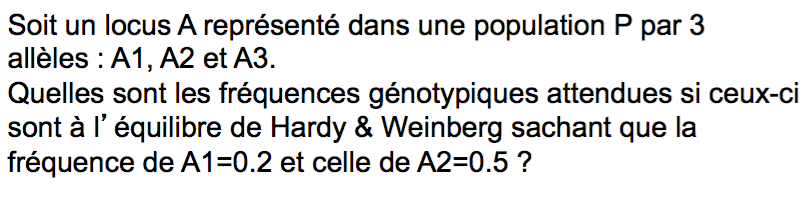
\includegraphics[width=100mm]{./ex3.png}
\end{figure}

Sachant que $A1=0.2$ et $A2=0.5$, on peut calculer la fréquence allélique de A3.

\begin{equation}
f(A3) = 1 - f(A1) - f(A2) = 1 - 0.2 - 0.5  = 0.3
\end{equation}

On sait que la population est à l'équilibre H-W et on demande les fréquence génotypiques attendues.

\begin{equation}
(p + q + r)^2 = p^2 + 2pq + q^2 + 2qr + r^2 + 2pr = 1
\end{equation}

On pose que A1 = q, A2 = p et A3 = r (peu d'importance)
\begin{equation}
f(A1A1) = q^2 = 0.2^2 = 0.04
\end{equation}

\begin{equation}
f(A2A2) = p^2 = 0.5 
\end{equation}

\begin{equation}
f(A3A3) = r^2 = 0.3^2 = 0.09
\end{equation}

\begin{equation}
f(A1A2) = 2 pq = 2 * 0.5 * 0.2 = 0.2
\end{equation}

\begin{equation}
f(A1A3) = 2qr = 2 * 0.2 * 0.3 = 0.12
\end{equation}

\begin{equation}
f(A2A3) = 2pr = 2*0.5*0.3 = 0.3
\end{equation}


\begin{figure}[H]
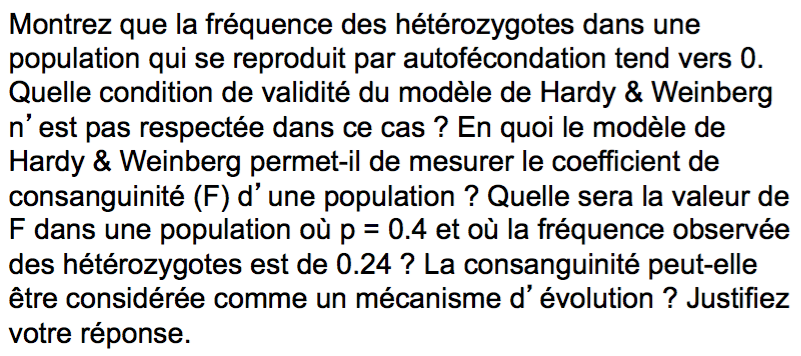
\includegraphics[width=100mm]{./ex9.png}
\end{figure}

En cas d'autofécondation, les hétérozygotes se reproduisent entre eux. De même pour les homozygotes dominants et récessifs.

De ce fait, à chaque génération, les hétérozygotes produiront 50\% d'homozygotes. Et les homozygotes produiront 100\%. \textbf{On perd donc 50\% d'hétérozygotes par génération !} Sur le long terme, les hétérozygotes vont donc disparaitre. La panmixie n'est pas respectée (accouplement non aléatoire).

On a la fréquence des hétérozygotes notée $H_0$ (fréquence attendue sous H-W):

\begin{equation}
H_0 = 2 pq = 2 *0.4*0.6 = 0.48
\end{equation}

Le coéfficient de consanguinité F:

\begin{equation}
F = \frac{H_0-H}{H_0} = \frac{0.48 - 0.24}{0.48} = 0.5
\end{equation}

où H est la fréquence observée.

\textbf{La consanguinité modifie les fréquences génotypiques (diminution des hétérozygotes) mais la fréquence allélique restera stable.} Ce n'est donc pas un mécanisme d'évolution en temps que tel. C'est une redistribution des allèles dans les génotypes.



\begin{figure}[H]
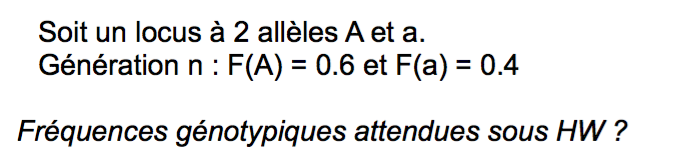
\includegraphics[width=100mm]{./ex5.png}
\end{figure}

On a déjà les fréquences alléliques, les fréquences génotypiques sont calculées immédiatement:

\begin{equation}
F(AA)_{att} = p^2 = 0.6 * 0.6 = 0.36
\end{equation}

\begin{equation}
F(Aa)_{att} = 2pq = 2*0.6*0.4 = 0.48
\end{equation}

\begin{equation}
F(aa)_{att} = q^2 = 0.4*0.4 = 0.16
\end{equation}

\begin{figure}[H]
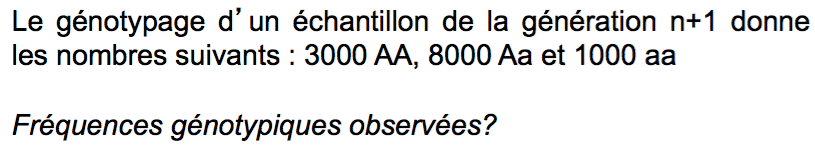
\includegraphics[width=100mm]{./ex6.png}
\end{figure}


\begin{equation}
F(AA)_{obs} = \frac{3000}{12000} = 0.25
\end{equation}

\begin{equation}
F(Aa)_{obs} = \frac{8000}{12000} = 0.67
\end{equation}

\begin{equation}
F(aa)_{obs} = \frac{1000}{12000} = 0.08
\end{equation}

Calculons \textbf{l'aptitude absolue W}:

\begin{equation}
W(AA) = \frac{F_{obs}}{F_{att}} = \frac{0.25}{0.36} = 0.69
\end{equation}
\begin{equation}
W(Aa) = \frac{0.67}{0.16} = 1.4
\end{equation}

\begin{equation}
W(aa) = \frac{0.08}{0.16} = 0.5
\end{equation}


l'aptitude relative w:

\begin{equation}
w(AA) = \frac{0.69}{1.4} = 0.49
\end{equation}

\begin{equation}
w(Aa) = \frac{1.4}{1.4} = 1
\end{equation}

\begin{equation}
w(aa) = \frac{0.5}{1.4} = 0.36
\end{equation}

et le coéfficient de sélection s:

\begin{equation}
s(AA) = 1 - w(AA) = 0.51
\end{equation}

\begin{equation}
s(Aa) = 1 - 1 = 0
\end{equation}

\begin{equation}
s(aa) = 1 - 0.36 = 0.64
\end{equation}


\begin{figure}[H]
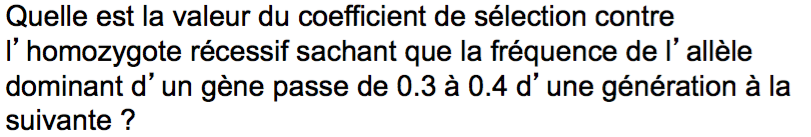
\includegraphics[width=100mm]{./ex7.png}
\end{figure}

On sait que p = 0.3 et p' = 0.4 car il s'agit de la fréquence de allèle dominant donné par l'énoncé. On cherche s.

\begin{equation}
\Delta p = p' - p = sp'q^2
\end{equation}

$q^2 = 0.49$ car q = 0.7 (= 1 - p).

\begin{equation}
0.1 = s 0.4 * 0.49
\end{equation}

\begin{equation}
s = \frac{0.1}{0.4*0.49} = 0.51
\end{equation}


\begin{figure}[H]
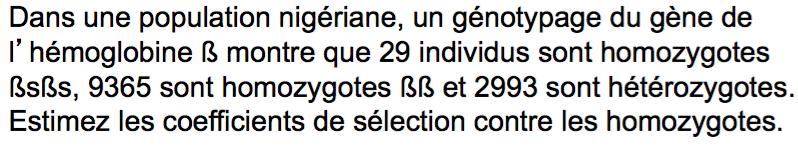
\includegraphics[width=100mm]{./ex8.png}
\end{figure}

Les coéfficients de sélection sont en relation avec l'aptitude relative $w = 1- s$.

On va donc calculer w. Mais pour cela, quelques étapes intermédiaires sont requises. On va d'abord calculé la fréquence génotypiques observées.

\begin{equation}
F_{obs}(\beta s \beta s) = \frac{29}{12387} = 0.00234116
\end{equation}

\begin{equation}
F_{obs}(\beta\beta s) = \frac{2993}{12387} = 0.24162428
\end{equation}

\begin{equation}
F_{obs}(\beta\beta) = \frac{9365}{12387} = 0.75684185
\end{equation}

Ensuite, on calcule la fréquence allélique:

\begin{equation}
F(\beta) = 0.75684185 + \frac{0.24162428}{2} = 0.87765399
\end{equation}

\begin{equation}
F(\beta s) = 1 - F(\beta) = 0.12234601
\end{equation}

Calculons les génotypes attendus sous H-W:

\begin{equation}
F_{att}(\beta s \beta s) = 0.12234601 * 0.12234601 = 0.01496854616
\end{equation}

\begin{equation}
F_{att}(\beta\beta s) = 2 * 0.87765399 * 0.12234601 = 0.21475492767
\end{equation} 

\begin{equation}
F_{att}(\beta\beta) = 0.87765399 * 0.87765399 =  0.77027652616
\end{equation}

Ensuite, on calcule l'aptitude absolue:

\begin{equation}
W(\beta s \beta s) = \frac{0.00234116}{0.01496854616} = 0.15640530315
\end{equation}

\begin{equation}
W(\beta\beta s) = \frac{0.24162428}{0.21475492767} = 1.1251163483
\end{equation}

\begin{equation}
W(\beta\beta) = \frac{0.75684185}{0.77027652616} = 0.98255863225
\end{equation}

les aptitudes relatives peuvent être calculées.

\begin{equation}
w(\beta s \beta s) = \frac{0.15640530315}{1.1251163483} = 0.13901255935
\end{equation}

\begin{equation}
w(\beta\beta s) = \frac{1.1251163483}{1.1251163483} = 1
\end{equation}

\begin{equation}
w(\beta\beta) = \frac{0.98255863225}{1.1251163483} = 0.87329513408
\end{equation}

\textbf{On est face à une sélection en faveur des hétérozygotes.}


Enfin, les coéfficient de sélection:

\begin{equation}
s(\beta s \beta s) = 1 - w(\beta s \beta s) = 0.86
\end{equation}

\begin{equation}
s(\beta\beta) = 1 - w(\beta\beta) = 0.12
\end{equation}



\pagebreak
\begin{figure}[H]
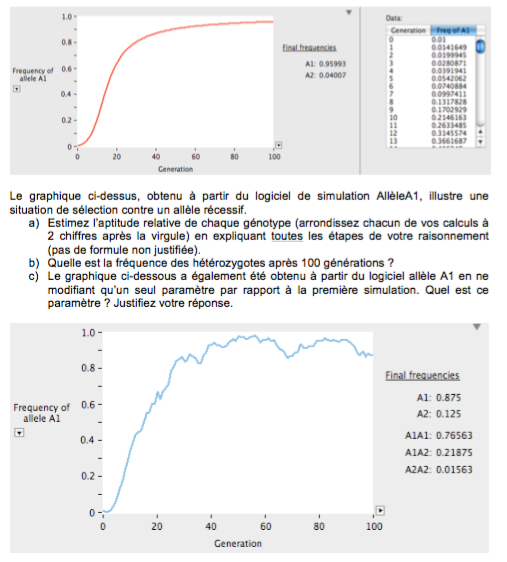
\includegraphics[width=140mm]{./ex4.png}
\end{figure}

Du premier graphique, on peut inférer que A1 est l'allèle dominant et que A2 est le récessif car on est en précense de sélection contre l'allèle récessif.

On est dans une simulation théorique. \textbf{Nous n'avons donc pas accès aux fréquences observées.} Le calcul de l'aptitude relative par l'aptitude aboslue n'est pas possible dans ce cas-ci.

Par contre, on peut calculer l'aptitude relative par le coéfficient de sélection:

\begin{equation}
w = 1 - s
\end{equation}

On peut calculer s par cette formule:

\begin{equation}
\Delta p = p' - p = sp'q^2
\end{equation}

\begin{equation}
p = 0.01 \Rightarrow q = 0.99 \Rightarrow q^2 = 0.9801
\end{equation}


\begin{equation}
0.0141649 - 0.01 = s * 0.0141649 * 0.9801
\end{equation}

\begin{equation}
s = \frac{0.0041649}{0.01388301849} = 0.3
\end{equation}

Donc,

\begin{equation}
w(A2A2) = 0.7
\end{equation}
\begin{equation}
w(A1A2) = 1
\end{equation}
\begin{equation}
w(A1A1) = 1
\end{equation}

La fréquence des hétérozygotes est données par 2pq et les valeurs sont données à la génération 100.

\begin{equation}
f(A1A2) = 2 * 0.95993 * 0.04007 = 0.0769287902
\end{equation}

Sur le deuxième graphique, on observe des oscillations, fluctuations aléatoires. C'est typiquement dû au fait qu'on considère une population de taille finie (et non plus infinie). C'est le phénomène de dérive génique.

\begin{figure}[H]
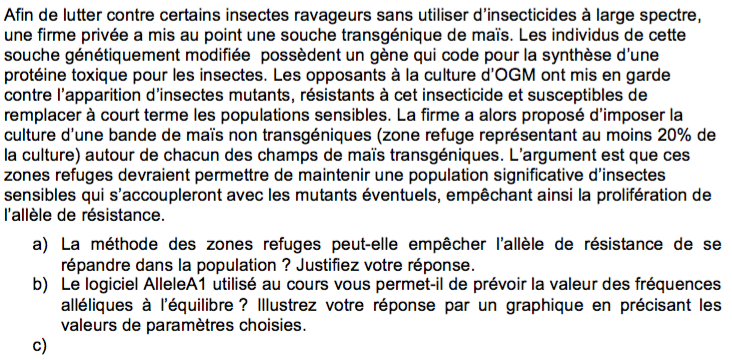
\includegraphics[width=100mm]{./ex10.png}
\end{figure}

Il est raisonable de penser que la population est homogène et \textbf{qu'on a une sélection contre l'homozygote récessif ou l'allèle dominant.} Si l'allèle de résistance est dominant, on aura pas beaucoup d'impact. En revanche, si l'allèle de résistance est récessif, cela va retarder la généralisation de l'allèle de résistance. Si on a migration entre les deux populations, la zone refuge est efficace. Cela permet d'éviter que l'allèle soit fixé et reste très fréquent.

On peut choisir dans le programme, une aptitude de 1 pour le génotype résistant et une aptitude de 0.2 pour le non résistant. Et donc en définitive, l'allèle résistant va disparaitre.

\begin{figure}[H]
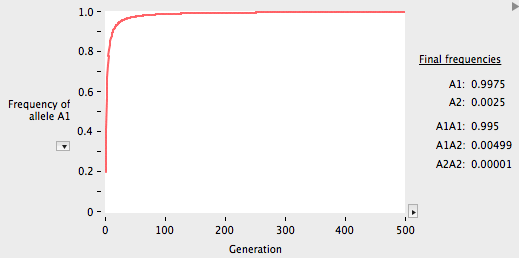
\includegraphics[width=100mm]{./s15.png}
\end{figure}

\begin{figure}[H]
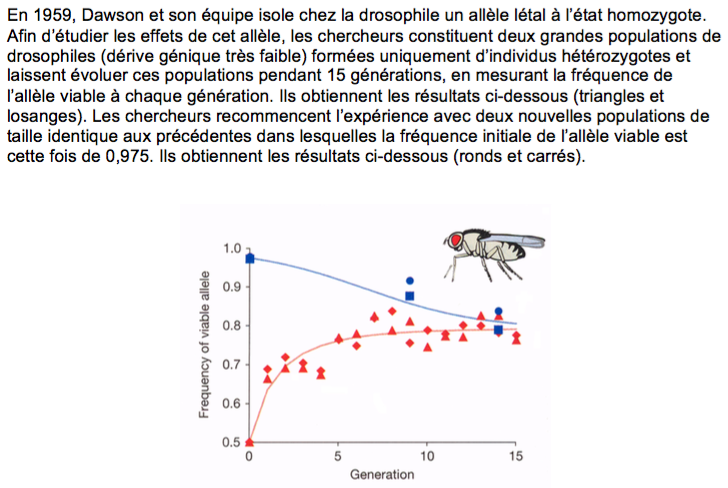
\includegraphics[width=100mm]{./ex11.png}
\end{figure}

\begin{figure}[H]
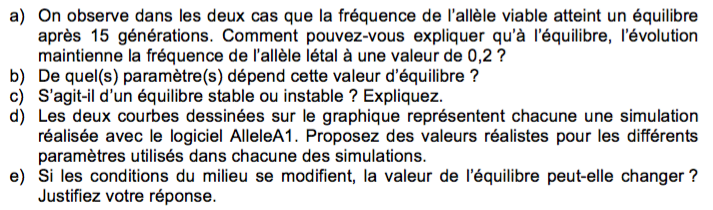
\includegraphics[width=100mm]{./ex12.png}
\end{figure}

Tout d'abord, \textbf{un allèle létal est d'officie récessif.} Donc l'allèle normal est dominant.
On est en précense de sélection en faveur des hétérozygotes. En effet, les individus hétérozygotes voient leur allèle récessif létal non exprimé. Il est donc tout a fait possible d'avoir un équilibre à 0.8 (voir section associée).

La valeur d'équilibre dépend des coéfficients de sélection s1 et s2. S1 est le coéfficient de sélection pour l'homozygote dominant et s2 le coéfficient de sélection pour l'homozygote récessif. Si s1 et s2 ne sont pas égales, la valeur d'équilibre est donnée par :

\begin{equation}
p* = \frac{s2}{s1+s2}
\end{equation}

si ils sont égales, la valeur d'équilibre est égale à 0.5. C'est un équilibre stable, un polymorphisme équilibré à contrario à l'équilibre instable qui est présent lors d'une sélection contre l'hétérozygote.

pour la courbe rouge, on a $f_{départ}=0.5$, une aptitude de 0 pour l'homozygote récessif, une aptitude de 1 pour l'hétérozygote et une aptitude de 0.75 (disons) pour l'homozygote dominant. Pour la courbe bleue, il n'y a que la fréquence de départ qui change, $f_{départ}=0.975$.

Effectivement, si les conditions du milieu change, la valeur d'équilibre change, le coéfficient de sélection se modifie.



\pagebreak

\begin{figure}[H]
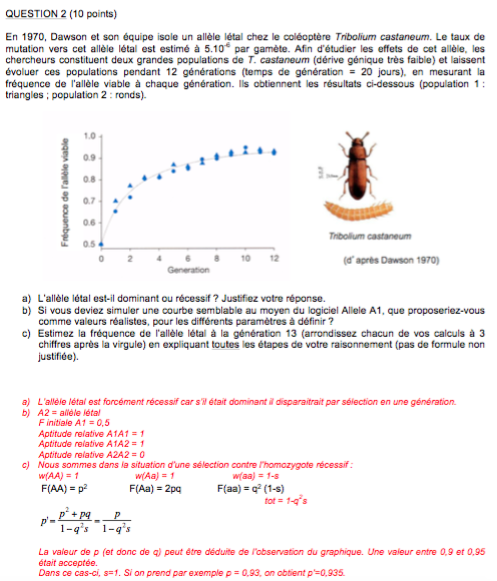
\includegraphics[width=170mm]{./ex13.png}
\end{figure}

\section{Ecart 2: la dérive génique}

Nous allons maintenant considérer une taille de population finie (et non plus infinie). La dérive génique se caractérise par la fluctuation des fréquences alléliques dans une population due à la variation aléatoire du succès reproducteur des individus. Plus la taille de la population est petite, plus la dérive génique est importante. De plus, celle-ci ne dirige pas l'avolution dans une direction déterminée en raison de ces fluctuations aléatoires (qu'on ne peut pas prédire). Elle a pour conséquence une perte de variation génétique au sein des populations. 

\begin{figure}[H]
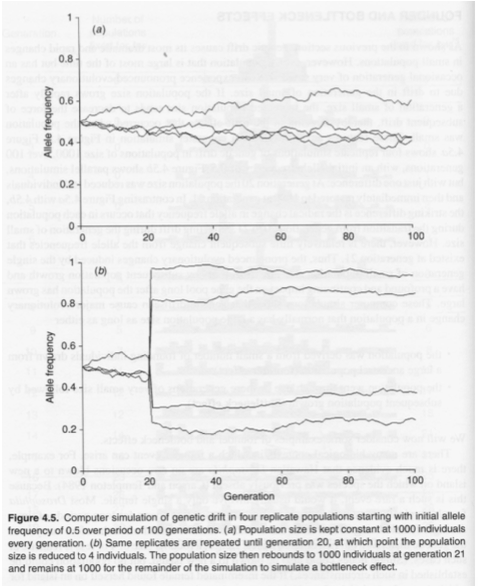
\includegraphics[width=100mm]{./s16.png}
\caption{Effet fondateur et bottleneck}
\end{figure}

On observe un goulot d'étranglement. A cause d'une catastrophe, la taille de la population peut diminuer brusquement.

Un tel cas de réduction importante de taille sur une seule ou quelques générations peut se présenter lorsqu’un petit groupe d’individus issus d’une grande population fondent une nouvelle population de grande taille, on parle alors \textbf{d’effet fondateur} (founder effect). Par contre, si une grande population passe par une réduction de taille importante pendant une ou quelques générations, avant de retrouver rapidement sa taille initiale, on parle d’effet \textbf{bottleneck.}

\subsection{Exercices}

\begin{figure}[H]
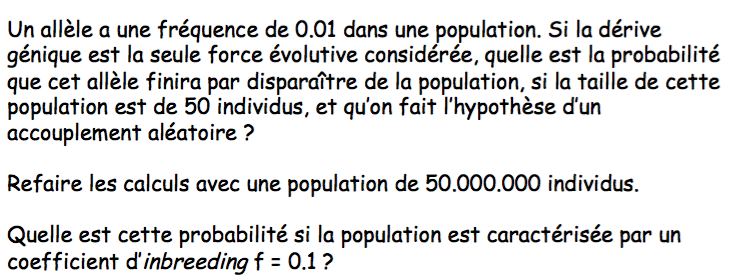
\includegraphics[width=100mm]{./ex14.png}
\end{figure}

On a un allèle de fréquence 0.01 noté A1. Donc A2, l'autre allèle à une fréquence de 0.99. \textbf{On aura une probabilité de 99\% que l'allèle disparaitra dans la population (1\% de chance qu'il soit fixé dans la population).} En effet, vu qu'on ne peut pas prédire au départ la direction de la fluctuation. Chaque allèle a une probabilité égale de se reproduire. \textbf{La vitesse de disparition est uniquement dépendante de sa fréquence de départ.} On considère qu'il n'y a pas de mutation ni de sélection.

Si la population est de 50 000 000 individus, la probabilité reste inchangée parce que le raisonnement est basé sur la fréquence de l'allèle dans la population au départ. Ce qui va changer est la vitesse de disparition de l'allèle, plus lente (car la force de la dérive génique est plus faible dans une grande population). Le temps de disparition de l'allèle sera beaucoup plus long.


\begin{figure}[H]
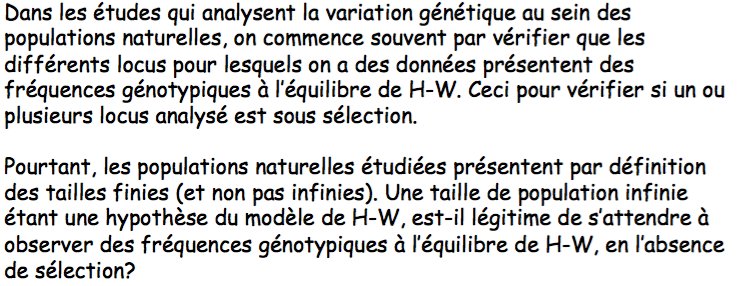
\includegraphics[width=100mm]{./ex15.png}
\end{figure}

Pour vérifier si une population est à l'équilibre Hardy-Weinberg, et donc pour obtenir les fréquences génotypiques attendues et ainsi les comparés avec celles observées, on a besoin des fréquences alléliques de la population. D'ou viennent ces fréquences ? Elles sont déduites des fréquences génotypiques observées, de la génération qu'on est en train d'étudier. On étudie donc pas l'évolution des fréquences alléliques au cours du temps. On ne travaille qu'avec une génération, celle qu'on étudie. Pour que la population soit à l'équilibre, il faut avoir des accouplements aléatoires. Si c'est le cas, les fréquences génotypiques vont correspondre aux fréquences génotypiques attendues sous H-W. Et donc on prend les fréquences alléliques de la même génération que les fréquences génotypiques. Si pas de sélection et accouplements aléatoires, alors équilibre H-W. Donc cela a un sens, pas de variation des fréquences allélique sur une seule génération.

\pagebreak

\begin{figure}[H]
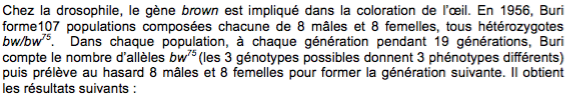
\includegraphics[width=100mm]{./ex16.png}
\end{figure}

\begin{figure}[H]
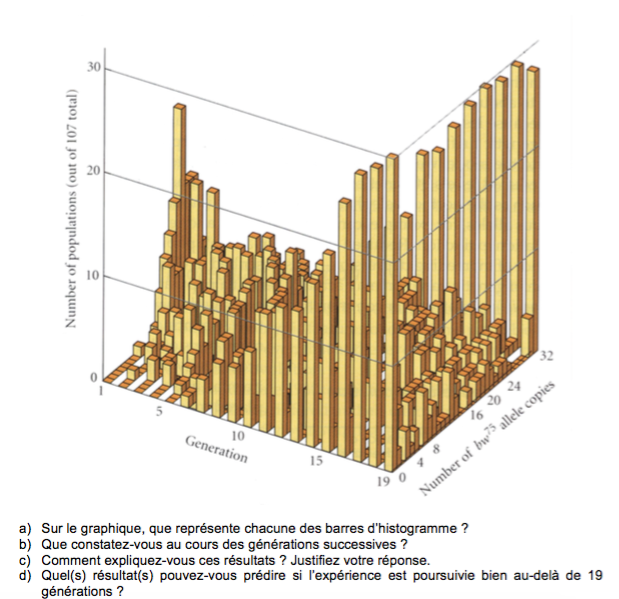
\includegraphics[width=100mm]{./ex17.png}
\end{figure}

Chaque barre représente un nombre de population à une génération donné.
Lors de la première génération, beaucoup de populations ont 32 copies de l'allèle bw75.

Au cours des générations, le nombre de populations qui avaient soit aucun allèle bw75 soit 32 allèles bw75 est augmenté. Il y a 50\% des deux allèles pour toutes ces populations à la première génération. Au fur et à mesure, il y a fixation d'un des deux allèles. La diversité génétique s'appauvrit au cours du temps.

Comment expliquer ces résultats ? La dérive génique. On est en précense de petites populations, on s'attend donc à une dérive génique forte. La fluctuations des fréquences alléliques est forte. On ne va pas dans une direction évolutive déterminée. On ne peut pas prédire la direction de l'évolution. A la fin, la majorité des populations n'ont plus qu'un des deux allèles.

Si l'expérience est poursuivie, toutes les populations seront soit dans le cas de fixation de l'allèle bw75 soit dans le cas de disparition de l'allèle bw75.

\pagebreak

\section{Ecart 3: déséquilibre de liaison}
Lorsqu'il y a deux locus à deux allèles sur le même chromosome, il peut se produire un phénomène de recombinaison. Le taux de recombinaison r est la probabilité d'avoir une recombinaison sur le chromosome de ces deux locus. Dès lors, de nouveaux génotypes font leur apparition dans la population.

le déséquilibe de liaison peut être calculé à la génération suivante t:

\begin{equation}
D_t = D_0(1-r)^t
\end{equation}

Cela permet de mesurer l'association entre deux locus. L'association maximum à un indice de 0.25.

\begin{figure}[H]
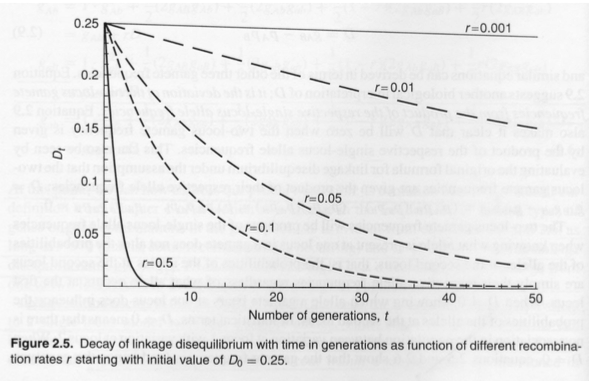
\includegraphics[width=100mm]{./s17.png}
\caption{Evolution de D au cours du temps}
\end{figure}

Le déséquilibre de liaison est une conséquence de forces évolutives principalement. Elle en résulte en un changement des fréquences gamétiques de la population.

\subsection{Exercices}

\begin{figure}[H]
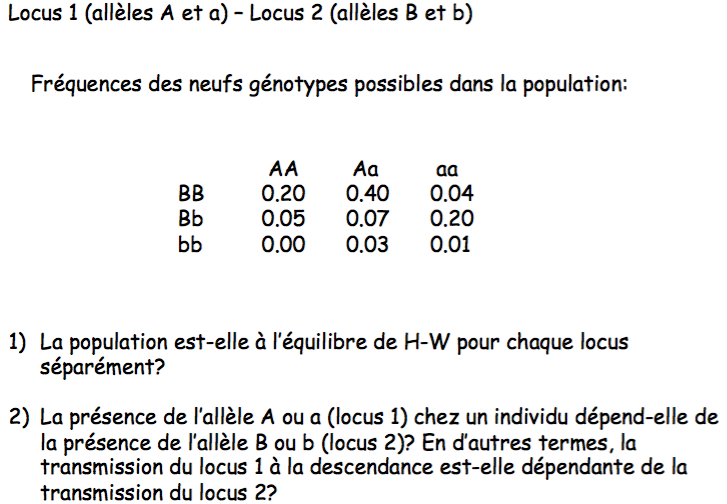
\includegraphics[width=100mm]{./ex18.png}
\end{figure}

On va commencer par le locus 1:

\begin{equation}
f(AA) = 0.25, f(Aa) = 0.5, f(aa) = 0.25
\end{equation}

La fréquence des allèles:

\begin{equation}
f(A) = 0.25 + \frac{0.5}{2} = 0.5
\end{equation}

\begin{equation}
f(a) = 1 - f(A) = 0.5
\end{equation}

\begin{equation}
f_{att}(AA) = 0.5^2 = 0.25
\end{equation}

\begin{equation}
f_{att}(Aa) = 2 * 0.5 * 0.5 = 0.5
\end{equation}

\begin{equation}
f_{att}(aa) = 0.5^2 = 0.25
\end{equation}

Le premier locus est à l'équilibre H-W.

Pour le deuxième locus:

\begin{equation}
f(BB) = 0.64, f(Bb) = 0.32, f(bb) = 0.04
\end{equation}

La fréquence des allèles:

\begin{equation}
f(B) = 0.64 + \frac{0.32}{2} = 0.8
\end{equation}

\begin{equation}
f(b) = 1 - f(B) = 0.2
\end{equation}

\begin{equation}
f_{att}(BB) = 0.8^2 = 0.64
\end{equation}

\begin{equation}
f_{att}(Bb) = 2 * 0.8 * 0.2 = 0.32
\end{equation}

\begin{equation}
f_{att}(bb) = 0.2^2 = 0.04
\end{equation}

Le deuxième locus est à l'équilibre H-W. \textbf{Donc la population est à l'équilibre d'H-W.}


Y-a-t-il une association entre les deux locus ? Est-ce que la transmission de l'un influence la transmission de l'autre ? 

Dans quel cas ils seraient transmis de manière indépendante ? Si les deux locus sont sur deux chromosomes différents. Si l'un influence la transmission de l'autre, une hypothèse possible serait qu'ils seraient sur le même chromosome. 

Si les locus sont indépendants, on peut calculer la fréquence génotypique attendues en faisant le produit des fréquences des génotypes pris séparement:


\begin{equation}
f_{att}(AA/BB) = f(AA) + f(BB) = 0.25 * 0.64 = 0.16
\end{equation}

Or on observe pas 0.16 dans le tableau mais 0.2. Donc, la fréquence observée n'est pas égale à la fréquence attendue.

On peut faire la même démarche pour une autre génotype:

\begin{equation}
f_{att}(Aa/BB) = 0.5 * 0.64 = 0.32
\end{equation}

Encore une fois la fréquence attendue est différente de celle observée. \textbf{On peut en conclure que les deux locus sont liés, associés. Leur transmission n'est pas indépendante.}



\begin{figure}[H]
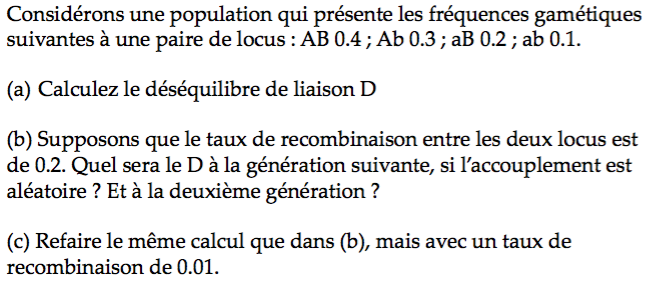
\includegraphics[width=100mm]{./ex19.png}
\end{figure}

Ici, nous avons affaire à des fréquences gamétiques. Nous allons premièrement calculer les fréquences alléliques (\textbf{somme des fréquences gamétiques}).

\begin{equation}
f(A) = g(AB) + g(Ab) = 0.4 + 0.3 = 0.7
\end{equation}

\begin{equation}
f(B) = g(AB) + g(aB) = 0.4 + 0.2 = 0.6
\end{equation}

On peut maintenant calculer D, le déséquilibre de liaison à la génération actuelle. \textbf{C'est la fréquence gamétique observée moins la fréquence gamétique attendue (produit des fréquences alléliques attendues).}

\begin{equation}
D_0 = g(AB) - (f(A) * f(B)) = 0.4 - (0.7*0.6) = -0.02
\end{equation}

A la génération suivante, en précense d'accouplement aléatoire, le déséquilibre de liaison est:

\begin{equation}
D_1 = D_0(1-r)^t = -0.02(1-0.2)^1 = -0.016
\end{equation}

En une génération, le déséquilibre de liaison à diminuer (il se rapproche de 0).

A la deuxième génération:
\begin{equation}
D_2 = D_0(1-r)^t = -0.02(1-0.2)^2 = -0.0128
\end{equation}

ou en réétulisant la valeur calculée précédemment:

\begin{equation}
D_2 = D_1(1-r)^t = -0.016(1-0.2) = -0.0128
\end{equation}

\pagebreak

\begin{figure}[H]
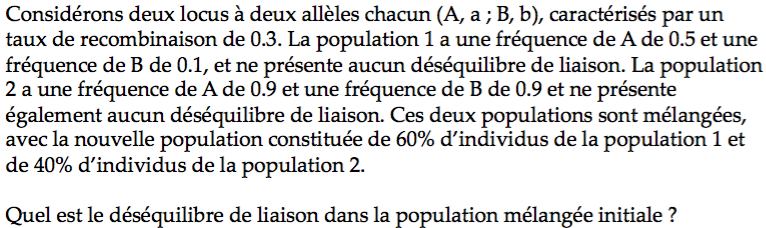
\includegraphics[width=100mm]{./ex20.png}
\end{figure}


\begin{equation}
D = g(AB) - (f(A)*f(B))
\end{equation}

On a besoin de la fréquence gamétique et des fréquences alléliques correspondante pour calculer le déséquilibre de liaison. Dans la population mélangée, on sait qu'on a 60\% d'individus de la population 1 et 40\% d'individus de la population 2.

Calculons premièrement la fréquence allélique dans la population finale en respectant les proportions.

\begin{equation}
f(A) = 0.6*f_1(A) + 0.4*f_2(A) = 0.6*0.5 + 0.4*0.9 = 0.66
\end{equation}

\begin{equation}
f(B) = 0.6*f_1(B) + 0.4*f_2(B) = 0.6*0.1 + 0.4*0.9 = 0.42
\end{equation}

Il ne reste plus que la fréquence gamétique. Pour cela, on utilise la formule du déséquilibre de liaison, et on sait qu'il vaut 0.

On commence par la population 1:

\begin{equation}
D = g(AB) - (f(A)*f(B)) = 0 
\end{equation}

\begin{equation}
g_1(AB) = (f(A)*f(B)) = 0.5 * 0.1 = 0.05
\end{equation}

Pour la population 2:

\begin{equation}
g_2(AB) = (f(A)*f(B)) = 0.9 * 0.9 = 0.81
\end{equation}

On calcule enfin les fréquences gamétiques dans la population mélangée:

\begin{equation}
g(AB) = 0.6 * 0.05 + 0.4 * 0.81 = 0.35
\end{equation}

Nous pouvons calculer la déséquilibre de liaison:

\begin{equation}
D = g(AB) - (f(A)*f(B)) = 0.35 - (0.66 * 0.42) = 0.077
\end{equation}

Au départ, il n'y avait pas de déséquilibre de liaison entre les deux locus dans les deux populations. Une fois qu'on les mélange, un déséquilibre apparait (assez élevé). Comment peut on l'expliquer ? C'est lié au fréquence alléliques. En effet, elles sont différentes dans les deux populations. Donc les fréquences gamétiques à l'équilibre vont être différentes. Les fréquences gamétiques ne vont plus correspondre au fréquence allélique de la population finale. On observe une association des deux locus car on a mélanger deux populations de fréquences alléliques différentes.


\pagebreak
\section{Ecart 4: accouplements non aléatoires}

\subsection{Accouplements préférentiels entre individus apparentés}

Comme ce sont des individus apparentés dont on parle, on est alors en précense \textbf{d'accouplements consanguins}. La conséquence de cela est une {diminution de la fréquence génotypique des hétérozygotes dans la population.}. Le \textbf{coéfficient (indice) de consanguinité} f permet de montrer le taux de diminution d'hétérozygote par rapport au taux normal \textbf{d'une population} (attendu sous H-W).

\begin{equation}
f = 1 - \frac{H_O}{H_{HW}}
\end{equation}

avec $H_0$ les fréquences hétérozygotes observées et $H_{HW}$ les fréquences attendues sous Hardy-Weinberg.

Il existe aussi le coéfficient d'inbreeding F qui se calcule à partir d'arbre généalogique, pédigré. \textbf{F d'un individu est la probabilité d'avoir un homozygote}.

\begin{figure}[H]
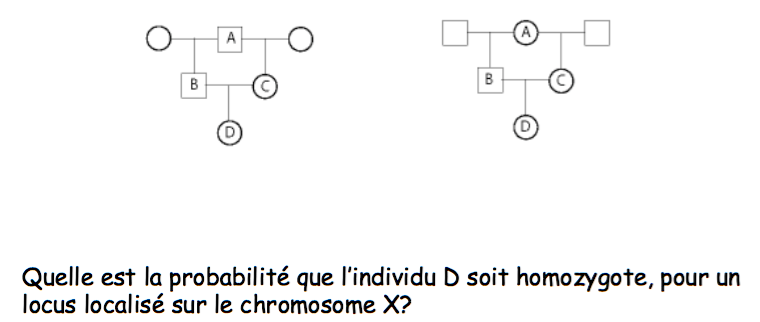
\includegraphics[width=110mm]{./ex21.png}
\end{figure}

Les individus femelles sont représenté par des ronds et les individus mâles par des carrés. Dans cet exercice, on parle d'un locus localisé sur le chromosome X, chromosome sexuel. Les allèles sont tous différents à la première génération car on ne sait pas ce qui s'est passé avant.

Pour la premier pedigré, La femmelle à gauche est $X_1X_2$, A est un male $X_3Y$ et la femelle de droite est $X_4X_5$. Quel est la probabilité de $X_3$ d'être transmis à B ? 0\% car A transmet déjà Y. D a 0\% de chance d'être $X_3X_3$. F=0. On ne parle pas de $X_1$ et $X_2$ car imaginons qu'elle transmet $X_1$, il faudrait que C aie aussi un $X_1$ (pour être homozygote) ce qui n'est pas possible. Par contre, C pourrait avoir $X_3$.


Pour le deuxième pedigré, A est une femelle $X_1X_2$. Probabilité que $X_1$ soit transmis à B ? 50\% et quelle est la probabilité que B transmet $X_1$ à D ? 100\%. Quelle est la probabilité que $X_1$ soit transmis à C? 50\% et quelle est la probabilité de transmission à D ? 50\%

On a donc 0.5 * 0.5 * 0.5 * 1 pour $X_1$ = $\frac{1}{8}$. Il y a également la probabilité de transmission de $X_2$ qui vaut aussi $\frac{1}{8}$. Donc F = $\frac{1}{8}$ + $\frac{1}{8}$ = $\frac{1}{4}$

\pagebreak

\begin{figure}[H]
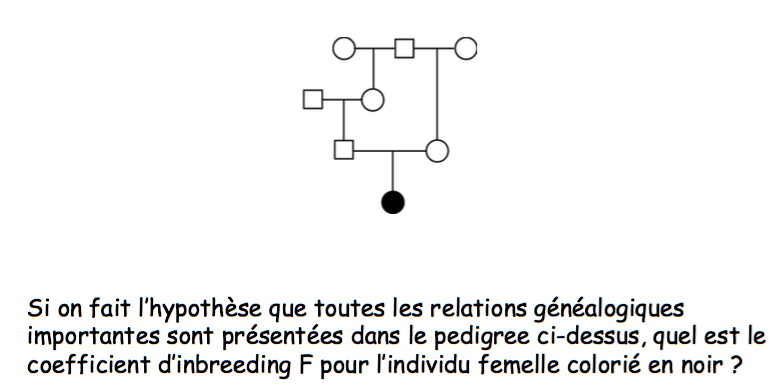
\includegraphics[width=110mm]{./ex22.png}
\end{figure}

On ne parle plus de X et Y car on n'est plus sur des chromosomes sexuelles.

Pour l'homme à la première génération, on a Aa. A a une probabilité de 50\% d'être transmis aux femelles de la génération suivante. 50\% pour être transmis au mâle suivant et enfin 50\% qu'il soit transmis à la femelle coloriée. Même chose pour l'autre descendant femelle. Même raisonnement pour le petit "a". 

\begin{equation}
F = (\frac{1}{2})^5 + (\frac{1}{2})^5 = \frac{1}{16}
\end{equation}

\subsection{Accouplements sélectifs}

\subsubsection{Entre phénotypes semblables}
L'accouplement est préférentiel entre individus dont le phénotype se ressemble. Ce phénomène peut être inconscient, préférence alimentaire pour qu'il y a cet accouplement. Il n'y a pas forcément attirance entre les deux individus.

Quel est l'impact sur les fréquences alléliques et génotypiques ? 

Le cas extrème est que les individus AA s'accouplement entre eux ainsi que les Aa et les aa (accouplement 100\% sélectif).

\begin{itemize}
\item fréquence génotypique: diminution des hétérozygotes \textbf{uniquement pour les locus impliqués dans le phénotype en question.}
\item fréquence allélique: stable, ne change pas.
\end{itemize}

Attention, pour deux locus, cela peit créer un déséquilibre de liaison et le maintenir. Il y a également une évolution des gamétiques au cours du temps.

Si on attend suffisamment longtemps, on aura plus d'hétérozygotes mais des que homozygotes.

\begin{figure}[H]
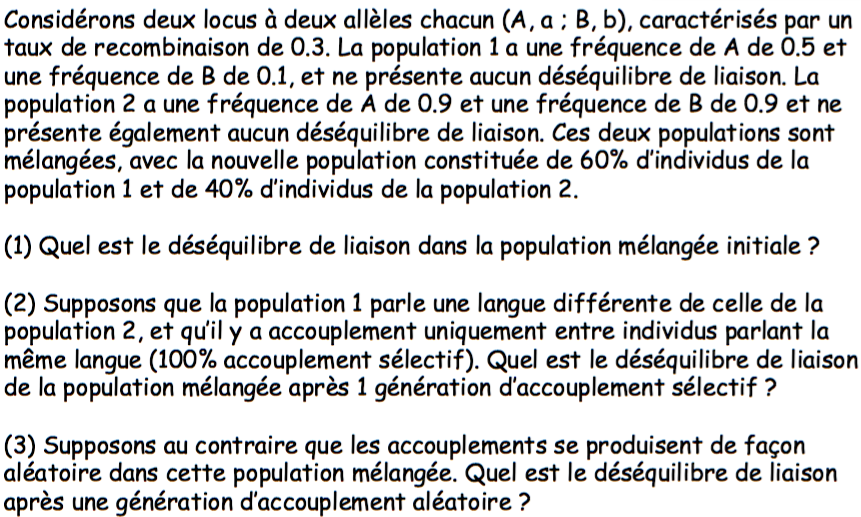
\includegraphics[width=110mm]{./ex23.png}
\end{figure}

Nous avons déjà résolu le (1) auparavant.

Pour la (2), pourquoi on a un accouplement 100\% sélectif ? Les individus d'une population vont s'accoupler avec les individus de la même population. Vont-ils jouer un rôle dans la définition du phénotype ? Le génotype influence la langue parlée ? Les deux locus n'ont rien avoir avec la langue et donc l'accouplements sélectif. En effet, la langue a une origine culturelle et non génotypique.On ne peut pas utiliser la formule vu au cours car elle n'est valable qu'en cas d'accouplement aléatoire. Les deux populations restent isolées. Le déséquilibre de liaison ne va pas évoluer. \textbf{Le déséquilibre de liaision est égale à 0.077 (comme à (1)).}

Dans le (3), on peut utiliser cette fois-ci la formule:

\begin{equation}
D = D_0 * (1-r)^t = 0.77 * (1-0.3) = 0.054
\end{equation}

\subsubsection{Entre phénotypes différents}
Les fréquences alléliques évoluent jusqu'à l'équilibre (f(A) = 0.5 et f(a) = 0.5). On a une augmentation des hétérozygotes pour les locus impliqués dans le phénotype considéré.

\pagebreak
\subsection{Exercices}

\begin{figure}[H]
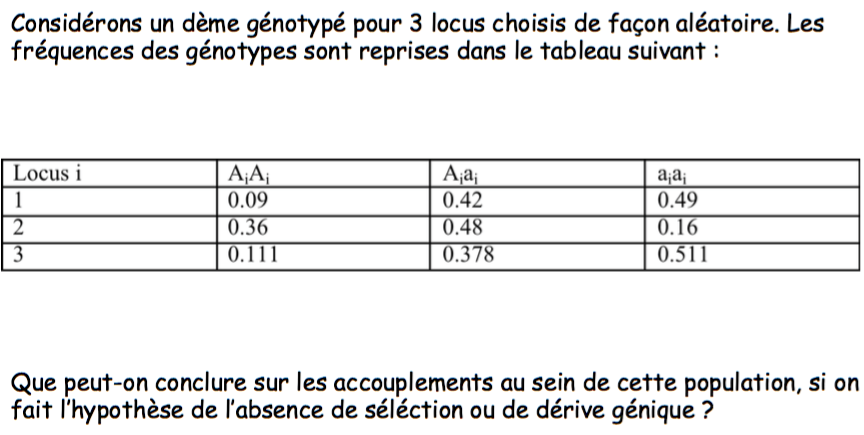
\includegraphics[width=110mm]{./ex24.png}
\end{figure}

Différents accouplement ont différent effet sur les fréquence génotypiques. Ici, on a un tableau référencant les fréquences génotypiques. Pour savoir quel est l'accouplement, il faut calculer les fréquences attendues sous H-W.

Pour le locus 1:

\begin{equation}
f(A) = 0.09 + \frac{0.42}{2} = 0.3
\end{equation}

\begin{equation}
f(a) = 1 - f(A) = 0.7
\end{equation}

\begin{equation}
f_{att}(AA) = 0.3^2 = 0.09
\end{equation}

\begin{equation}
f_{att}(Aa) = 2*f(A)*f(a) = 2*0.3*0.7 = 0.42
\end{equation}

\begin{equation}
f_{att}(aa) =  = 0.7^2 = 0.49
\end{equation}

Le premier locus est à l'équilibre H-W. Donc, pour le premier locus, nous avons des accouplements aléatoires pour ce locus.

Pour le locus 2:

\begin{equation}
f(A) = 0.36 + \frac{0.48}{2} = 0.6
\end{equation}

\begin{equation}
f(a) = 1 - 0.6 = 0.4
\end{equation}

\begin{equation}
f_{att}(AA) = 0.6^2 = 0.36
\end{equation}

\begin{equation}
f_{att}(Aa) = 2*f(A)*f(a) = 2*0.6*0.4 = 0.48
\end{equation}

\begin{equation}
f_{att}(aa) =  = 0.4^2 = 0.16
\end{equation}

Le locus 2 est également à l'équilibre H-W.

Pour le locus 3:

\begin{equation}
f(A) = 0.111 + \frac{0.378}{2} = 0.3
\end{equation}

\begin{equation}
f(a) = 1 - 0.3 = 0.7
\end{equation}

\begin{equation}
f_{att}(AA) = 0.3^2 = 0.09
\end{equation}

\begin{equation}
f_{att}(Aa) = 2*f(A)*f(a) = 2*0.3*0.7 = 0.42
\end{equation}

\begin{equation}
f_{att}(aa) =  = 0.7^2 = 0.49
\end{equation}

Le locus 3 n'est pas à l'équilibre H-W. On a une diminution des hétérozygotes. On est soit dans des accouplements consanguins soit dans des accouplements sélectifs à phénotypes semblables. Or, \textbf{seul le locus 3 est impacté donc on est en précense d'accouplements sélectifs à phénotypes semblables}

\begin{figure}[H]
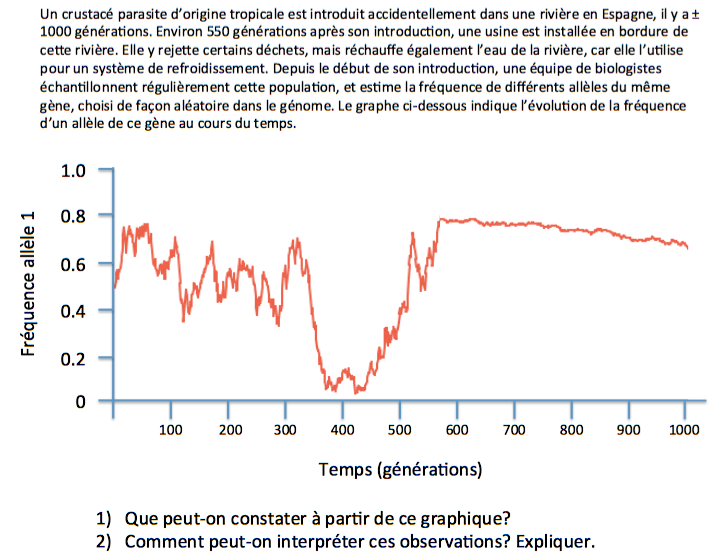
\includegraphics[width=160mm]{./ex25.png}
\end{figure}


On a une stabilisation de la fréquence de l'allèle, elle devient plus stable au cours du temps. La diversité génétique a baissé. Pourquoi? \textbf{La taille de la population augmente} vu que l'eau se rechauffe et que c'est une espèce tropicale. La taille de la population a tendance à stabiliser la fréquence car la dérive génique est plus faible. 

\pagebreak

\begin{figure}[H]
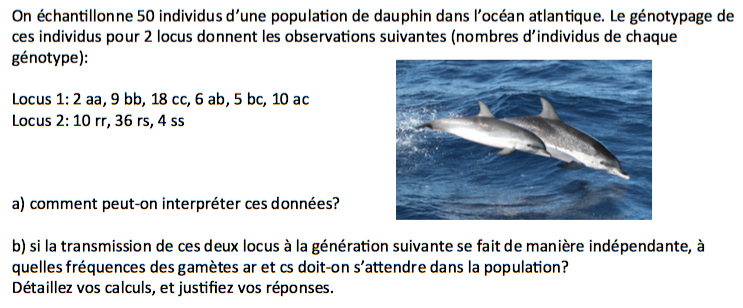
\includegraphics[width=140mm]{./ex27.png}
\end{figure}

Pour le locus 1, il y a 3 allèles. 2 allèles pour le locus 2.

Pour le locus 2, on a un excès d'hétérozygotes. Pour le locus 1 on a un déficit d'hétérozygotes (faire calcul). Comment peut on l'interpréter ? 


\begin{itemize}
\item Une première hypothèse serait un accouplement sélectif pour phénotypes semblables pour le locus 1 et un accouplement sélectif pour phénotypes différents pour le locus 2.

\item Une deuxième hypothèse: sélection en faveur des hétérozygotes pour le locus 2. \textbf{Si la sélection impacte un locus, elle ne va pas agir sur l'ensemble du génome.} Sélection en faveur des homozygotes pour le locus 1. \textbf{On peut envisager deux types de sélection pour des locus differents.}

\item On peut imaginer un accouplement sélectif pour phénotypes differents pour le locus 2 et une sélection en faveur des homozygotes pour le locus 1.
\end{itemize}

La dérive génique se voit à travers les générations et pas à une génération. Ce déficit/excès ne peut donc pas s'expliquer par dérive génique. On ne peut pas non plus donner de conclusion sur la liaison des deux locus par déséquilibre de liaison (pas assez d'information dans l'énoncé).


Quelle serait les fréquences des gamètes ar et cs dans la population ?
Comme la transmission des deux locus est fait de manière indépendante, la fréquence des gamètes est le produit des fréquences.

\begin{equation}
g(ar) = f(a)*f(r) = 0.56*0.2 = 0.112
\end{equation}

\begin{equation}
g(cs) = f(c)*f(s)
\end{equation}

\pagebreak

\begin{figure}[H]
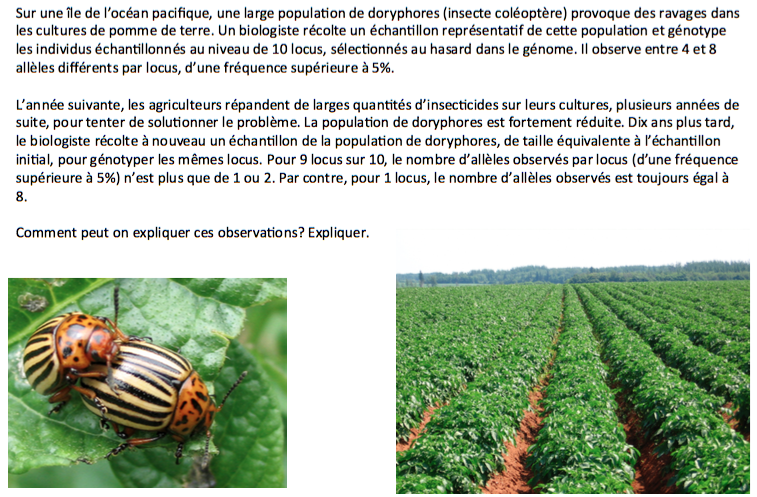
\includegraphics[width=140mm]{./ex28.png}
\end{figure}

Les locus ont été choisi au hasard dans tout le génome. La sélection en faveur des hétérozygotes est peu probable puisque qu'on aurait échantilloné 9 locus sur 10 présentant sélection. Ce qui est fortuit.

La population est fortement réduite en raison de la mise en place d'insecticides. De ce fait, la dérive génique devient forte et fait évoluer la diversité génétique. On a une perte de fréquence pour 9 locus sur 10 à cause de la dérive génique. C'est cette hypothèse qu'on va privilégier.

\pagebreak

\begin{figure}[H]
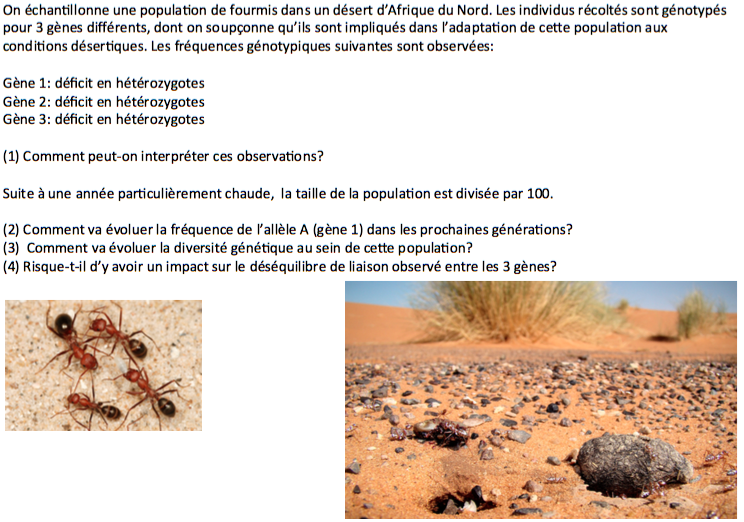
\includegraphics[width=140mm]{./ex29.png}
\end{figure}

Le déficit en hétérozygotes des trois gènes peut s'expliquer par un acccouplement consanguin (\textbf{la grande majorité des gènes au sein du génome présente un déficit en hétérozygotes}) ou une sélection en faveur des homozygotes. L'accouplement sélectif pour phénotypes semblables est moins plausible puisqu'on échantillonne 3 gènes aléatoirement.

\textbf{La dérive génique impacte tout le génome, la sélection impacte un ou plusieurs gènes mais pas tout le génome.}

La fréquence de l'allèle A va fluctuer plus fort en raison de la petite taille de la population. On ne peut pas prédire la direction de la force évolutive.

La diversité génétique va s'appauvrir, diminuer. La fluctuation va être grande et la probabilité qu'un allèle disparaisse est haute.

Oui, il y a un risque qu'il y aie un déséquilibre de liaison. La dérive génique change la fréquence allélique mais aussi gamétique. La dérive génique peut induire un déséquilibre de liaison.




\end{document}
